\documentclass[11pt]{article}
\usepackage[a4paper,margin=22mm,headheight=16pt]{geometry}
\usepackage{fontspec,xeCJK,xcolor,graphicx,enumitem,fancyhdr,titlesec}
\usepackage{hyperref}
\IfFontExistsTF{Times New Roman}{\setmainfont{Times New Roman}}{\setmainfont{TeX Gyre Termes}}
\IfFontExistsTF{FangSong}{\setCJKmainfont[AutoFakeBold=2]{FangSong}}{\IfFontExistsTF{仿宋}{\setCJKmainfont[AutoFakeBold=2]{仿宋}}{\IfFontExistsTF{FandolFang-Regular.otf}{\setCJKmainfont[AutoFakeBold=2]{FandolFang-Regular.otf}}{\setCJKmainfont{FandolSong-Regular.otf}}}}
\definecolor{ink}{HTML}{173747}\definecolor{accent}{HTML}{227E82}
\hypersetup{colorlinks=true,urlcolor=accent,linkcolor=accent}
\linespread{1.22}\setlength{\parindent}{0pt}\setlength{\parskip}{6pt}
\setlist[itemize]{leftmargin=1.4em,itemsep=3pt}
\titleformat{\section}{\large\bfseries\color{ink}}{}{0pt}{}
\titlespacing*{\section}{0pt}{14pt}{7pt}
\pagestyle{fancy}\fancyhf{}\lhead{\small OMNI LEARNING / 学习手册}\rhead{\small Source-grounded learning}\cfoot{\small\thepage}
\emergencystretch=2em\widowpenalty=10000\clubpenalty=10000
\newcommand{\Needspace}[1]{\par\begingroup\dimen0=#1\relax\vskip0pt plus\dimen0\penalty-100\vskip0pt plus-\dimen0\vskip\dimen0\penalty9999\vskip-\dimen0\vskip0pt\endgroup}
\begin{document}


{\LARGE\bfseries\color{ink} 洪武废相与治理难题}\par

2026-10-08 | Day02/30 | 阅读 8 分钟 + 练习 3 分钟\par\vspace{6pt}

\Needspace{5\baselineskip}\section*{今日导航}

今天回答：取消一个重要职位，是否就消除了它处理的问题？目标是理解洪武时期中央机构调整，并用“权力归属与事务处理”两条线分析。先回忆昨天：哪种说法是制度事实，哪种只是我们对后果的推论？

\Needspace{5\baselineskip}\section*{先核对发生了什么}

故宫博物院的中书省资料介绍，明初沿用中书省制度，洪武时期逐步调整，1380年罢中书省、废丞相，相关权力分给六部等机构。[S2] 今天保留这个核心事实，不要求记全部官名。还应注意：这一过程不是简单把现代公司的组织图套进古代国家，机构职责和政治关系有自己的历史背景。

\begin{center}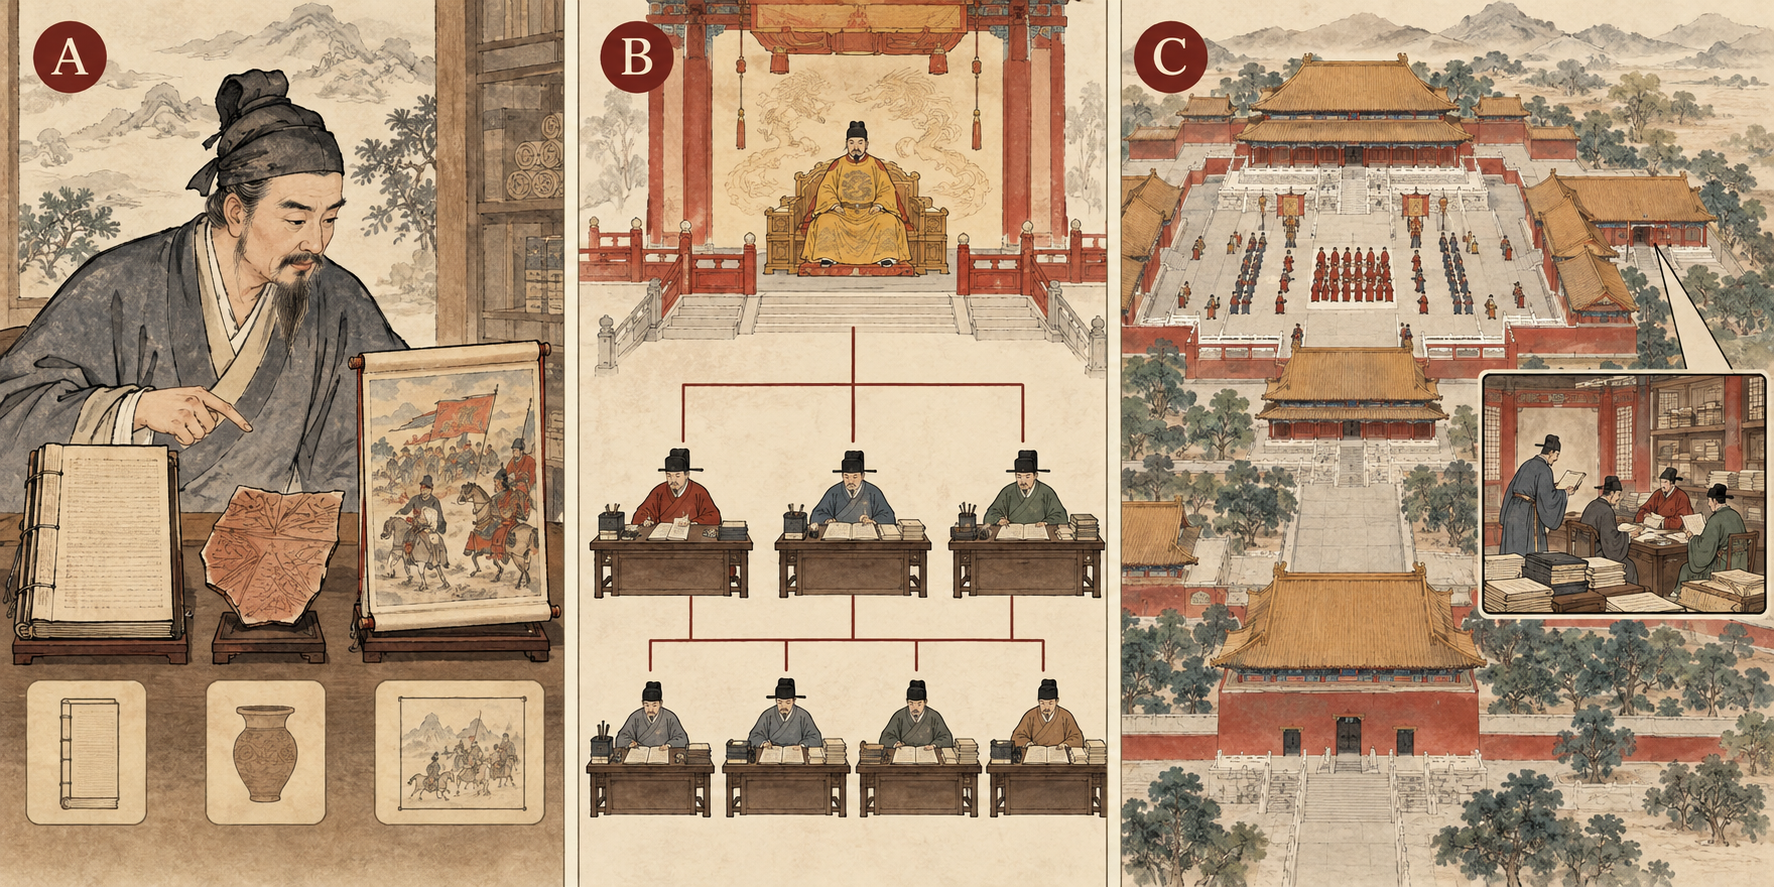
\includegraphics[width=\linewidth,height=0.26\textheight,keepaspectratio]{../assets/figure-e75918c40f59.png}\par

{\small 本课重点看 B 区。A 文字、器物与图像需要互证；B 思考决策和执行关系；C 区分宫城礼仪空间与日常政务。人物、服饰和机构排列均非史料复原。}\par

{\footnotesize AI生成教学示意，非实物照片、原始史料或官方架构。生成方式：内置文生图；提示词见仓库 docs/image-prompts.json。}\end{center}

\Needspace{5\baselineskip}\section*{权力集中与信息处理}

从权力归属看，皇帝减少了一个强势的中间枢纽；从事务处理看，奏章、协调和执行并不会因职位消失而自动消失。后一个判断是本课根据组织问题提出的分析视角，需要结合具体史料检验，不能冒充某位当事人的原话。

故宫的介绍也讨论了废相后辅助政务机制的变化。[S2] 学习时可以区分“制度规定谁有权”和“实际工作怎样被处理”。两者相关，却不是同一个问题。只说“皇权加强”会遗漏日常运转，只说“效率下降”又可能过早作出没有充分证据的评价。

图 B 是抽象的决策与执行关系，不是明代中央官制复原图。图中人物数量、服饰和层级不能用来背六部或判断真实机构。真正的机构关系应回到文字资料与专业研究核实。

\Needspace{5\baselineskip}\section*{用双栏法理解变化}

在纸上写两栏：左栏“谁决定”，右栏“谁处理”。把你读到的调整分别放进去；遇到两栏都受影响的变化，在中间画连接。这样能避免认为权力越集中，所有具体事务就一定越容易处理。

一个教学类比是团队负责人取消中间协调角色后，需要重新分配信息汇总和跨部门协调。但类比只帮助发现问题，不证明古代官员像现代员工一样行动。判断历史后果还要看不同皇帝、时期和机构如何实际运作。不要用一个看似通顺的组织学故事解释整个明代。

\Needspace{5\baselineskip}\section*{三分钟练习与自查}

请用三句话回答：发生了什么制度变化？它可能改变哪一种权力关系？它留下什么需要进一步研究的运行问题？

参考：第一句写1380年废中书省及丞相这一核心调整；第二句说明决策权更加向皇帝集中；第三句追问信息汇总和机构协调如何承担。自查第三句是否仍保留为问题，而不是写成“因此必然导致明亡”。从明初制度直跳数百年后的结果，缺少了大量中间证据。

\Needspace{5\baselineskip}\section*{复盘与明日连接}

历史中的制度既分配权力，也安排事务。认识变化要同时看规则、实际运行与后续调整，不用单一原因包办兴亡。明天从宫城空间观察另一种皇权表达：宏大的礼仪秩序与日常治理怎样联系，又怎样不同？

\Needspace{6\baselineskip}\section*{扩展学习 / Further reading}\small 以下为选读，不计入每日必做时间。\begin{enumerate}[leftmargin=1.6em]

\item [S1] \href{https://www.metmuseum.org/essays/ming-dynasty-1368-1644}{Ming Dynasty (1368–1644)} — 从文物与艺术观察明代，避免把宫廷与文人经验视为全部社会。\par The Metropolitan Museum of Art | 发布：2002-10-01 | 核验：2026-10-08

\item [S2] \href{https://www.dpm.org.cn/court/system/236406.html}{中书省} — 核对洪武时期机构调整，并把制度事实与作者的因果解释区分开。\par 故宫博物院 | 发布：未标注 | 核验：2026-10-08

\item [S3] \href{https://whc.unesco.org/en/list/439/}{Imperial Palaces of the Ming and Qing Dynasties} — 查看北京宫殿营建时间、轴线与礼仪空间；注意明清长期改建。\par UNESCO | 发布：未标注 | 核验：2026-10-08

\item [S4] \href{https://whc.unesco.org/en/list/1004/}{Imperial Tombs of the Ming and Qing Dynasties} — 从陵寝空间理解皇权表达，与宫殿材料交叉观察。\par UNESCO | 发布：未标注 | 核验：2026-10-08

\item [S5] \href{https://www.metmuseum.org/exhibitions/listings/2009/arts-of-the-ming-dynasty}{Arts of the Ming Dynasty} — 旧展览档案用于认识作品种类，不代表展览仍在开放。\par The Metropolitan Museum of Art | 发布：未标注 | 核验：2026-10-08

\end{enumerate}

\end{document}